Communication as mentioned before is a key part of AVs.
A \textit{Vehicular ad hoc network} (or VANET) is a proposed type of \textit{mobile ad hoc network} (called also MANET)
involving road vehicles.
This type of network permits vehicles to communicate with roadside equipment,
such as traffic lights, and with each other\cite{sheikh2019comprehensive}.
The main purpose of such technology is to generate security on the roads,
in this case security in terms of passengers and pedestrian safety.
The main components of VANET technology are: \textit{On-board unit (OBU)},
\textit{Road-side unit (RSU)}, \textit{Trusted Authority (TA)}.
The Trusted Authority acts as a key part in the VANET architecture,
as it is responsible for managing the security of the network and ensuring that all vehicles are authenticated
and authorized to communicate.

Communications are crucial for Autonomous Vehicles (AVs) to interact with other vehicles, infrastructure, and the cloud.
There may be many ways to categorize communications in AV devices.
One approach is based on the range of communication,
so a categorization that focus on the different distances covered by the communication.
Another approach can be based on the kind of subject involved in the communication,
so a categorization that focus on the type of interaction and the entities involved in the communication.
Range can classify communications in AVs as:
\begin{enumerate}
    \item \textbf{Short-range communication}
    \item \textbf{Medium-range communication}
    \item \textbf{Long-range communication}
\end{enumerate}

Or by the kind of subject involved in the communication:
\begin{enumerate}
    \item \textbf{Vehicle-to-Vehicle (V2V)}
    \item \textbf{Vehicle-to-Infrastructure (V2I)}
    \item \textbf{Vehicle-to-Everything (V2X)}
\end{enumerate}

In the following sections, more details for the different type of communication will be provided.

\subsection{Vehicle-to-Vehicle (V2V)}\label{subsec:vehicle-to-vehicle-(v2v)}

When speaking about Vehicle-to-Vehicle (V2V), the focus is on communications that happen between vehicles.
It obviously involves wireless communications between motor vehicles,
aiming primarily to prevent accidents by exchanging data such as position and speed.
This communication happens within an ad-hoc mesh network, which can either be fully connected or partially connected.
In both cases, messages can be relayed directly or through multiple paths,
ensuring robust communication even if some nodes fail.
While wired mesh networks were once expensive and challenging to implement,
wireless technologies, such as WPANs, have made them possible today\cite{arena2019overview}.

The advantages in terms of new functionalities and comfort offered to the drivers are clearly various.
Some examples of security-improving features created by exploiting V2V are the Blind Spot Detection (BSD) that warns the drivers about other vehicles of any type located out of sight,
the Forward Collision Warning System (FCWS), automatic emergency braking (AEB) and the Lane departure warning system (LDWS)\cite{arena2019overview}.

In terms of design,
the USDOT (Department of Transportation of the United States of America) has documented the security requirements of
systems and in particular, the need to define security network requirements for V2V and its supporting systems.

\subsection{Vehicle to Infrastructure (V2I)}\label{subsec:vehicle-to-infrastructure-(v2i)}
Vehicle to Infrastructure is another type of communication in Intelligent Transportation System (ITS)
that enables vehicles to communicate with roadside infrastructure, such as traffic lights, signs, and road sensors.

In this case, communication can vary greatly depending on the type of infrastructure with which you want to communicate.
It can be exploited to provide real-time traffic information, road condition updates, and other services to drivers,
representing the next evolution and a significant step towards the development of smart cities\cite{dot2024v2i}.

State and local agencies are expected to install V2I systems either alongside or integrated with existing ITS equipment.
As a result, many V2I deployments could be eligible for similar federal-aid programs as ITS,
provided the deploying agency meets certain requirements\cite{dot2024v2i}.

\subsection{Vehicle to Everything (V2X)}\label{subsec:vehicle-to-everything-(v2x)}

Vehicle-to-Everything (V2X) is a general communication model that generalizes Vehicle-to-Vehicle (V2V) and Vehicle-to-Infrastructure (V2I) systems,
incorporating interactions between vehicles and other entities, such as pedestrians (V2P)~\cite{vehicle-to-pedestrian}, roadside equipment (V2R)~\cite{vehicle-to-roadside}, and devices (V2D).
V2X, like V2V and V2I, aims to enhance road safety, focussing on vulnerable road users.

\begin{figure}[!htb]
    \centering
    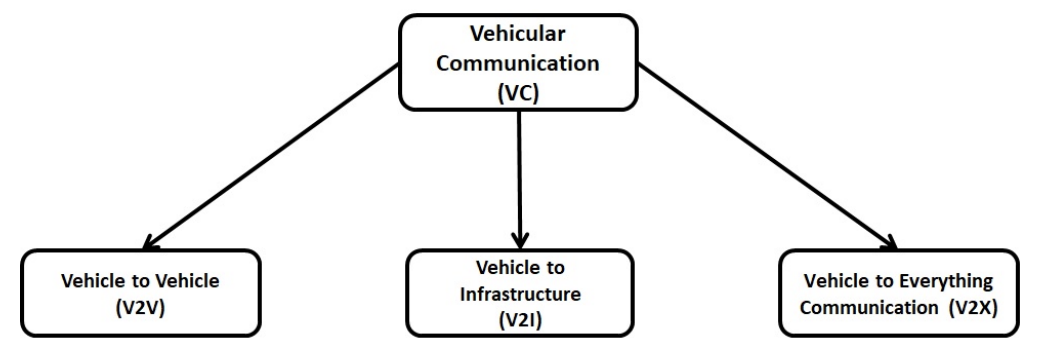
\includegraphics[width=0.7\linewidth]{figures/communication}
    \caption{VANETs}
    \label{fig:communication}
\end{figure}

\subsection{Controller Area Network bus}\label{subsec:canbus-communication}
Internal communications are managed by the Controller Area Network (CAN) bus.
CAN is the most common network topology
used for controlling industrial machinery
and widely used in the automotive industry also due to its cheapness and reliability.
It is a communication network that offers rapid communication among microcontroller
devices.
Each component in the network is connected to the bus and called node.
CAN permits these nodes to use a message-based protocol designed to
let all nodes receive and send messages on the network\cite{canbus}.
The CAN bus is a broadcast network,
meaning that all nodes on the network receive the message and require no authentication to receive the message,
that is hazardous in terms of security.
Due to its unsecure nature,
the CAN bus is vulnerable to cyber-attacks and is the standard interface that attackers use to inject attack messages into the
communication network.
It is required for a malicious attacker to have physical access to the vehicle to perform the attack, constraining the attacker to be near the target vehicle.
The exploitation in this case is only physical and not through the network;
in that case, the attacker can be located anywhere in the world.
Researchers tried
to evaluate some new technologies to detect the malicious code
and mitigate the attacks\cite{aldhyani2022attacks}\ref{subsec:artificial-intelligence}
using deep learning algorithms to detect the malicious code on the CAN bus.
The proposed systems have demonstrated effective detection of abnormal packets to safeguard the CAN bus.
Additionally,
they can be adapted to other security system designs within the complex infrastructures of autonomous vehicle networks,
ensuring more secure data processing.
